A test was performed to find the fiber length that optimizes the tritium detection efficiency. Two different lengths of scintillating fibers were considered in this study, $1~\meter$ and $20~\cm$ and two different tritium source activity were used, $0.5~\kilo\becquerel/\liter$ and $2.5~\kilo\becquerel/\liter$. As detected tritium counts is proportional to the active area, 5 detectors were simulated for the case of $0.20~\meter$ fiber length to normalize the study to the same active area. As the active area of the detector is related to its tritium detection efficiency, the advantage to use long fibers is their large active areas with a small number of cells, reducing the number of photosensors and, consequently, the price of the TRITIUM monitor. However, a smaller length of scintillating fibers reduce de photon absortion produced in the fibers, increasing the tritium detection efficiency per active area.

To find the scintillating fiber length that optimize the tritium detection efficiency, the Tritium-Aveiro prototype, consisting of a similar design as the TRITIUM-IFIC 2 prototype but with $360$ scintillating fibers of $2~\mm$ diameter, was simulated. All optical properties were included in this study in which the photon propagation was included.

The propagation of photons in scintillating fibers was studied. The number of photons produced in a scintillating fiber per tritium event was compared between all tritium events that reach the scintillating fiber and only those  tritium events the photons of which are detected in time coincidence by the photosensors, shown in Figure \ref{fig:PhotonsFibersYesNoPhotosensors}.

\begin{figure}[h]
\centering
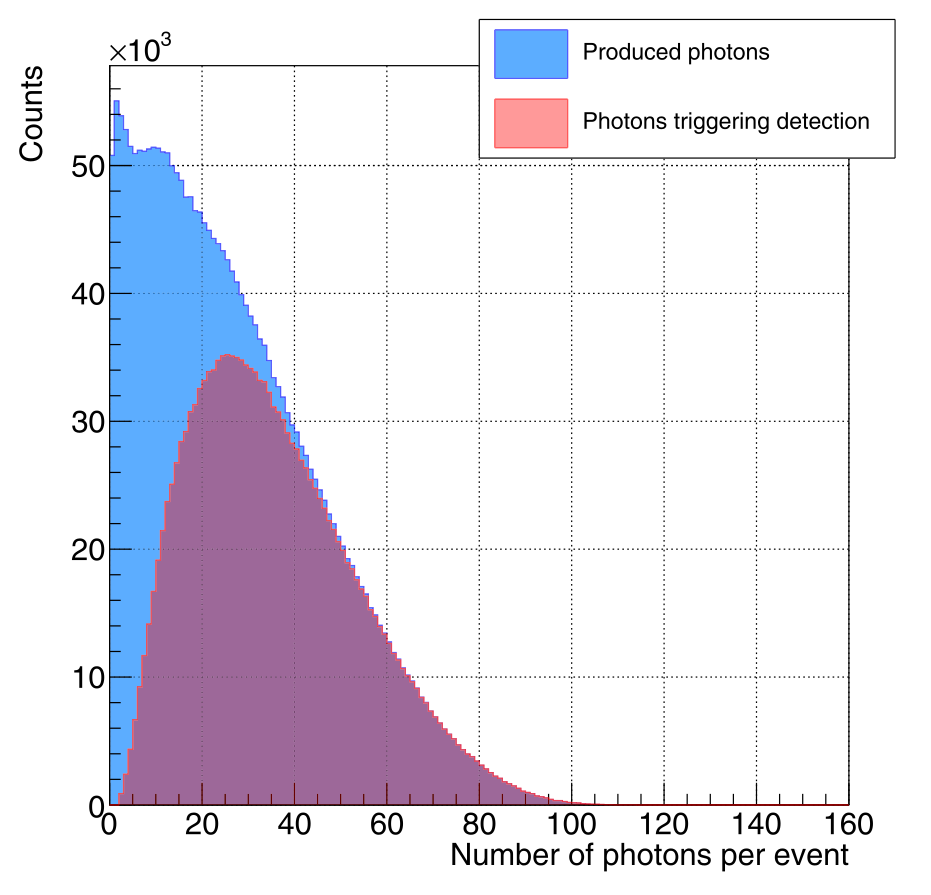
\includegraphics[scale=0.3]{Figures/8SimulationsResults/81TRITIUMDesign/813Length/CollectionPhotonsInFibers.png}
\caption{Number of photons produced in the fiber per tritium event for all tritium events that reach the fiber (blue histogram) and only for tritium events the photons of which are detected by photosensors (red histogram) \cite{SimulationPaperCarlos}.\label{fig:PhotonsFibersYesNoPhotosensors}}
\end{figure}

It can be seen that tritium events that produce a high number of photons are practically always detected but most of the events with fewer photons produced in the fibers are not detected, producing a peak centred of around $25$ photons.  

Regarding the fiber length study, the counts, integred over $60~\min$ and taken over a week, are shown in Figure \ref{fig:CountsOver60minDifferentLength} as a function of the time.

\begin{figure}[h]
\centering
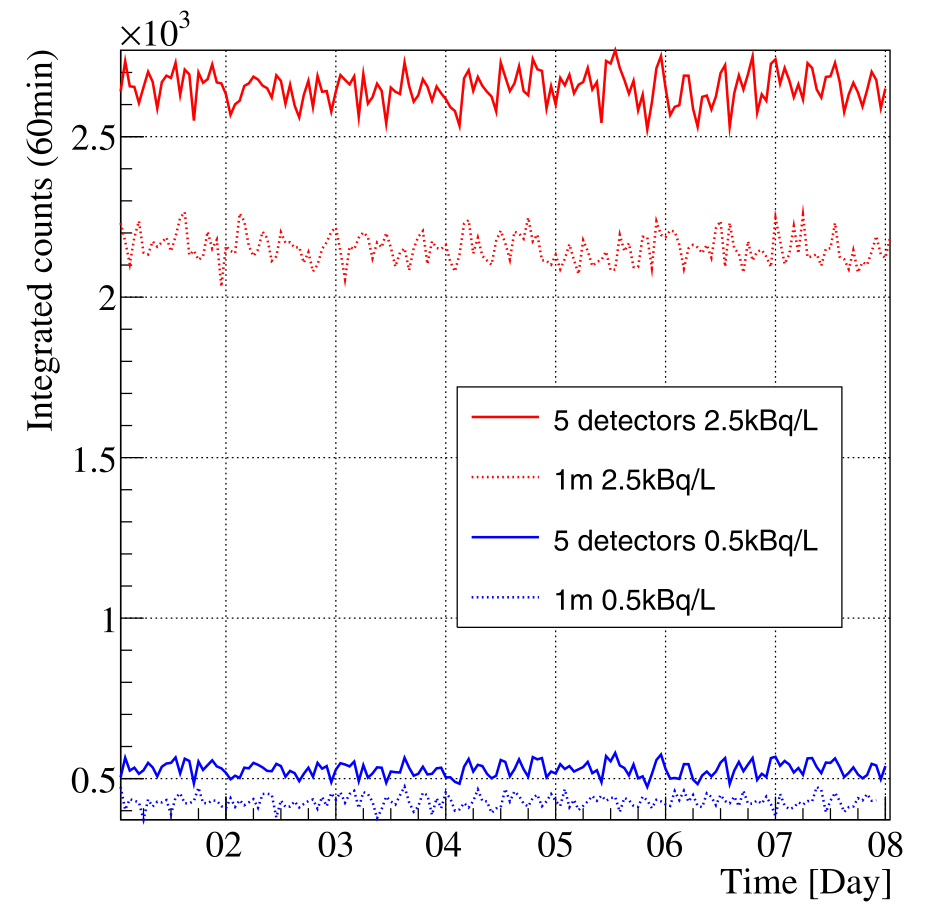
\includegraphics[scale=0.3]{Figures/8SimulationsResults/81TRITIUMDesign/813Length/2DifferentLength.png}
\caption{Counts integred over $60~\min$, normalized to the same active area and taken over a week for a fiber length of $1~\meter$, dashed lines, and $20~\cm$, solid lines and two different activities, $0.5~\kilo\becquerel/\liter$, blue lines, and $2.5~\kilo\becquerel/\liter$, red lines \cite{SimulationPaperCarlos}. \label{fig:CountsOver60minDifferentLength}}
\end{figure}

A larger signal is seen for shorter fiber lengths in both cases, producing a increasement in tritium detection efficiency of approximately $25\%$, principally caused by a lower absortion of photons in shorter scintillating fibers and the leakage of some photons due to a non-perfect photon collection in the fiber. In addition, non simulation effects like the dirty or mechanical imperfections of scintillating fibers increase accentuate this effect.